\documentclass[10pt,titlepage]{article}
\usepackage{fullpage}
\usepackage{listings}
\usepackage{graphicx}
\usepackage{float}

\begin{document}
  \title{Lab 4: iRobot Navigation in C}
  \author{Sam Mansfield and Toan Vuong\\
          TA: Hoekun Kim\\ 
          EECS149}
  \date{October 2nd, 2013}
  \maketitle

  \section{Introduction} 
  \ \ \ \ In this lab, we improved the iRobot's navigation system. By first designing an algorithm, then implementing it using state machines, we allowed the iRobot to get around obstacles to continue on its original direction. \\
  \section{Analysis}
    %Analysis of algorithm used
  \ \ \ \ Our algorithm is fairly simple. Our robot will start off moving forward. When it detects either an obstacle or a cliff, it will move backwards, turn right, then attempt to turn left to return to its original trajectory. If this fails because another obstacle is in the way, it will attempt the algorithm all over again. The figure below demonstrates this. \\
    \begin{figure}[H]
        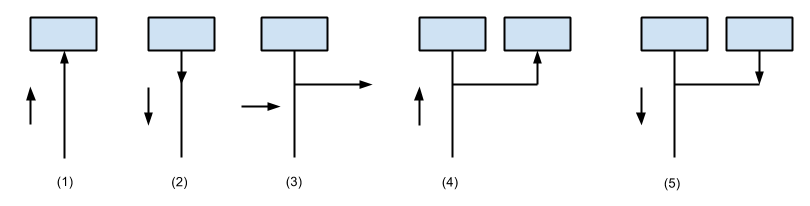
\includegraphics[keepaspectratio, width=1\textwidth]{../lab4_data/a.png}
        \caption{Algorithm Part 1. Single obstacles. Arrows denote direction of travel.}
    \end{figure}
  It works on the basis that, in order to return to the original direction, our robot must turn left once for every right turn it makes. This leaves the robot to move forward in its original trajectory. in its original orientation This means that we have to keep track of the number of obstacles that the robot has encoutered. Everytime we successfully dodge an obstacle, this obstacle counter decreases by one. \\
  \ \ \ \ In Figure 2,  our robot is in the process of avoiding an obstacle when it reaches another obstacle. In state (7), its obstacle count increases to 2. It begins the obstacle avoidance algorithm in (8), and (9). Figure 3 shows state (10), where the robot has successfully made two right turns, corresponding to two increments of the obstacle counter, and one left turn, corresponding to one decrement of the obstacle counter. \\
  \ \ \ \ Thus, in (11), when the robot makes the final left turn, the number of obstacles decreases to zero and it is back facing its original direction again.
    \begin{figure}[H]
        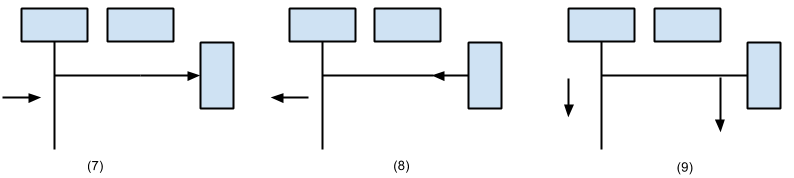
\includegraphics[keepaspectratio, width=1\textwidth]{../lab4_data/b.png}
        \caption{Algorithm Part 2. Encoutering an obstacle while avoiding the first. Arrows denote direction of travel.}
    \end{figure}
    \begin{figure}[H]
        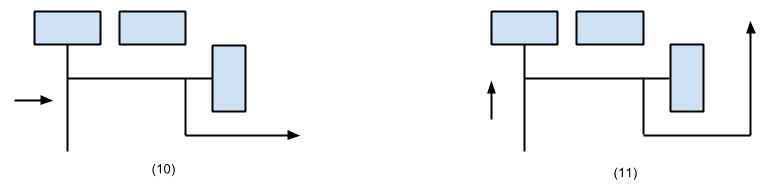
\includegraphics[keepaspectratio, width=1\textwidth]{../lab4_data/c.png}
        \caption{Algorithm Part 3. Recovery from both obstacles. Arrows denote direction of travel..}
    \end{figure}
    
     
    %State Machine 
  To accomodate this algorithm in the robot's states, we ended up adding two new states, BACK and TURNRIGHT. The BACK state goes backwards for 50 mm, the TURNRIGHT state makes a right turn. We reused the existing TURN state as a TURNLEFT. Figure 4 displays our final FSM.

  At the beginning of the lab we tried to create a more elaborate FSM and realized that we were actually making things more complicated to debug and therefore implement. By simplifying our design we created a better FSM. It was a little unclear if we were supposed to use the square pattern that initially boots up or to just make the robot go straight. Initially we created an obstacle avoidance algorithm that only worked for the square pattern. It was only later on that we realized that we were supposed to create an obstacle avoidance algorithm for a straight line.
    
    \begin{figure}[H]
      \centering
        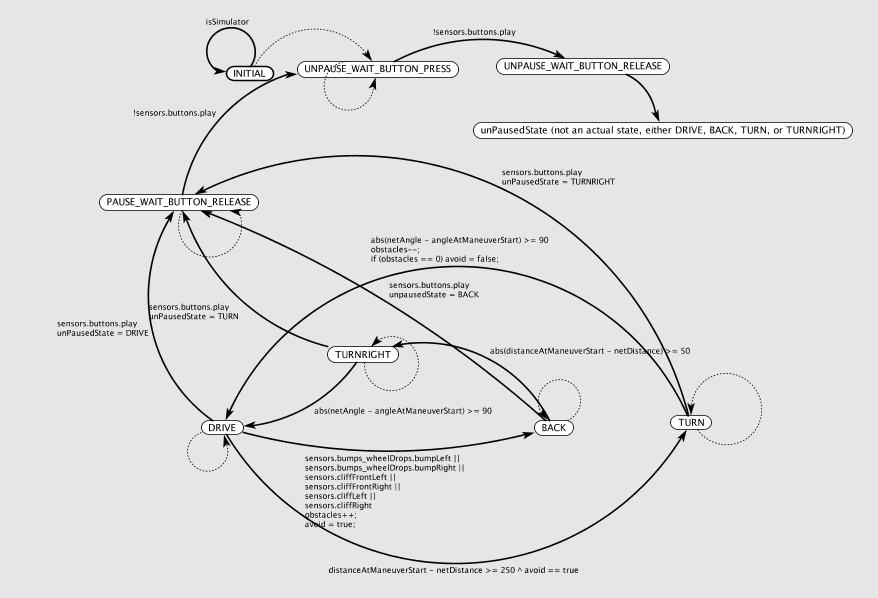
\includegraphics[width=1\textwidth]{../lab4_data/FSMLab4v2}
      \caption{Obstacle/Cliff avoidance FSM implemented in Lab 4}
    \end{figure}

  \section{Conclusion}
    Designing an obstacle/cliff avoidance algorithm was quite fun and rewarding when it actually worked. This was a very applicable problem for state machines and we can apply this technique to future problems that are similar in nature. This lab also helped us think about solving very simple human problems (avoiding an obstacle) step by step so that it can be applied to a robot.
\end{document}
